\section{Wissensdarstellung in wissensbasierten Systemen}

Wissensbasierte Informationsverarbeitung basiert auf der Vorstellung, dass viele Probleme nur l�sbar sind, wenn man Erfahrung mit dem Problem und den L�sungsm�glichkeiten daf�r hat. Dies wirft die Frage auf: Wie stellen wir Wissen so dar, dass es von Computern verstanden und zur Probleml�sung verwendet werden kann?

Wissen wird dabei als Klassen, Kategorien und Konzepte mit Hierarchien, Zusammensetzungen und Klassifikationen dargestellt. Dies ist eine ontologische Erfassung einer Anwendungsdom�ne bekannt. Diese Art der Datenmodellierung l�sst sich am besten mit einer Mindmap vergleichen (siehe Abb.~\ref{fig:mind-map-example}).

\begin{figure}[H]
    \centering
    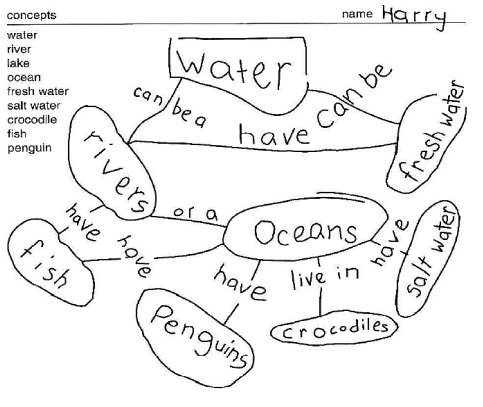
\includegraphics[width=0.52\textwidth]{figures/kap6/mind-map.png}
    \caption{Beispiel einer Mindmap von einem Grundsch�ler}
    \label{fig:mind-map-example}
\end{figure}

Diese Klassen, Kategorien und Konzepte werden letztlich in der Implementierung durch programmtypische Datenstrukturen wie Objekt-Arrays und Pointer abstrahiert (Abb.~\ref{fig:knowledge-darsetllung-ebenen}).

\begin{figure}[H]
    \centering
    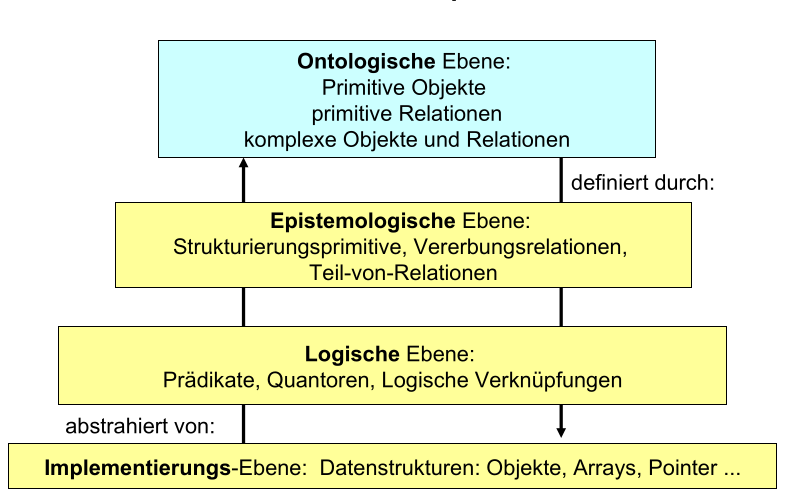
\includegraphics[width=0.8\textwidth]{figures/kap6/ebenen-wissendarstellung.png}
    \caption{Ebenen der Wissensrepr�sentation}
    \label{fig:knowledge-darsetllung-ebenen}
\end{figure}

Es gibt viele M�glichkeiten, Wissen explizit darzustellen. Eine Anwendung kann logikbasierte Ans�tze wie Fakten und Regeln verwenden. Andere k�nnen Rahmen und F�lle oder strukturierte Vererbungsnetze �hnlich objektorientierter Modelle verwenden.